\begin{frame}[t]{TS912 - Recherche} 

    Eine einfache Recherche für uns zu einem Hersteller, hier zum Beispiel ST.
    \href{https://www.st.com/en/amplifiers-and-comparators/ts912.html}{https://www.st.com/en/amplifiers-and-comparators/ts912.html}


    \begin{spacing}{0.9} \begin{tiny}
        \begin{table}[h!]
          \begin{tabular}{p{5cm} p{5cm}}
              \begin{minipage}{0.5\textwidth}
                  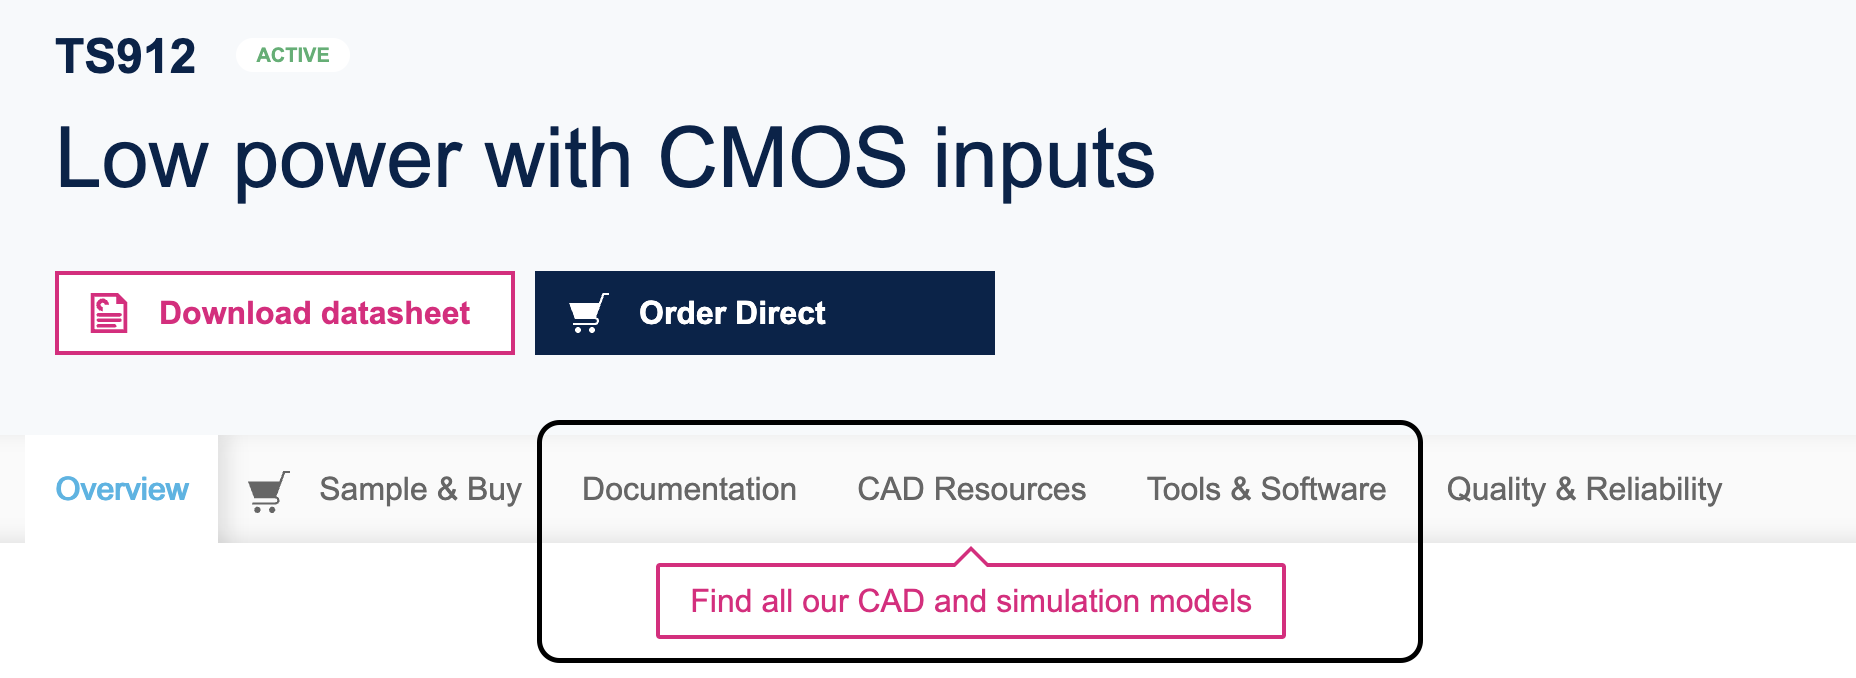
\includegraphics[width=\linewidth]{pictures/spice_model_search.png}
              \end{minipage} 
              &
              \begin{minipage}{0.5\textwidth}
                  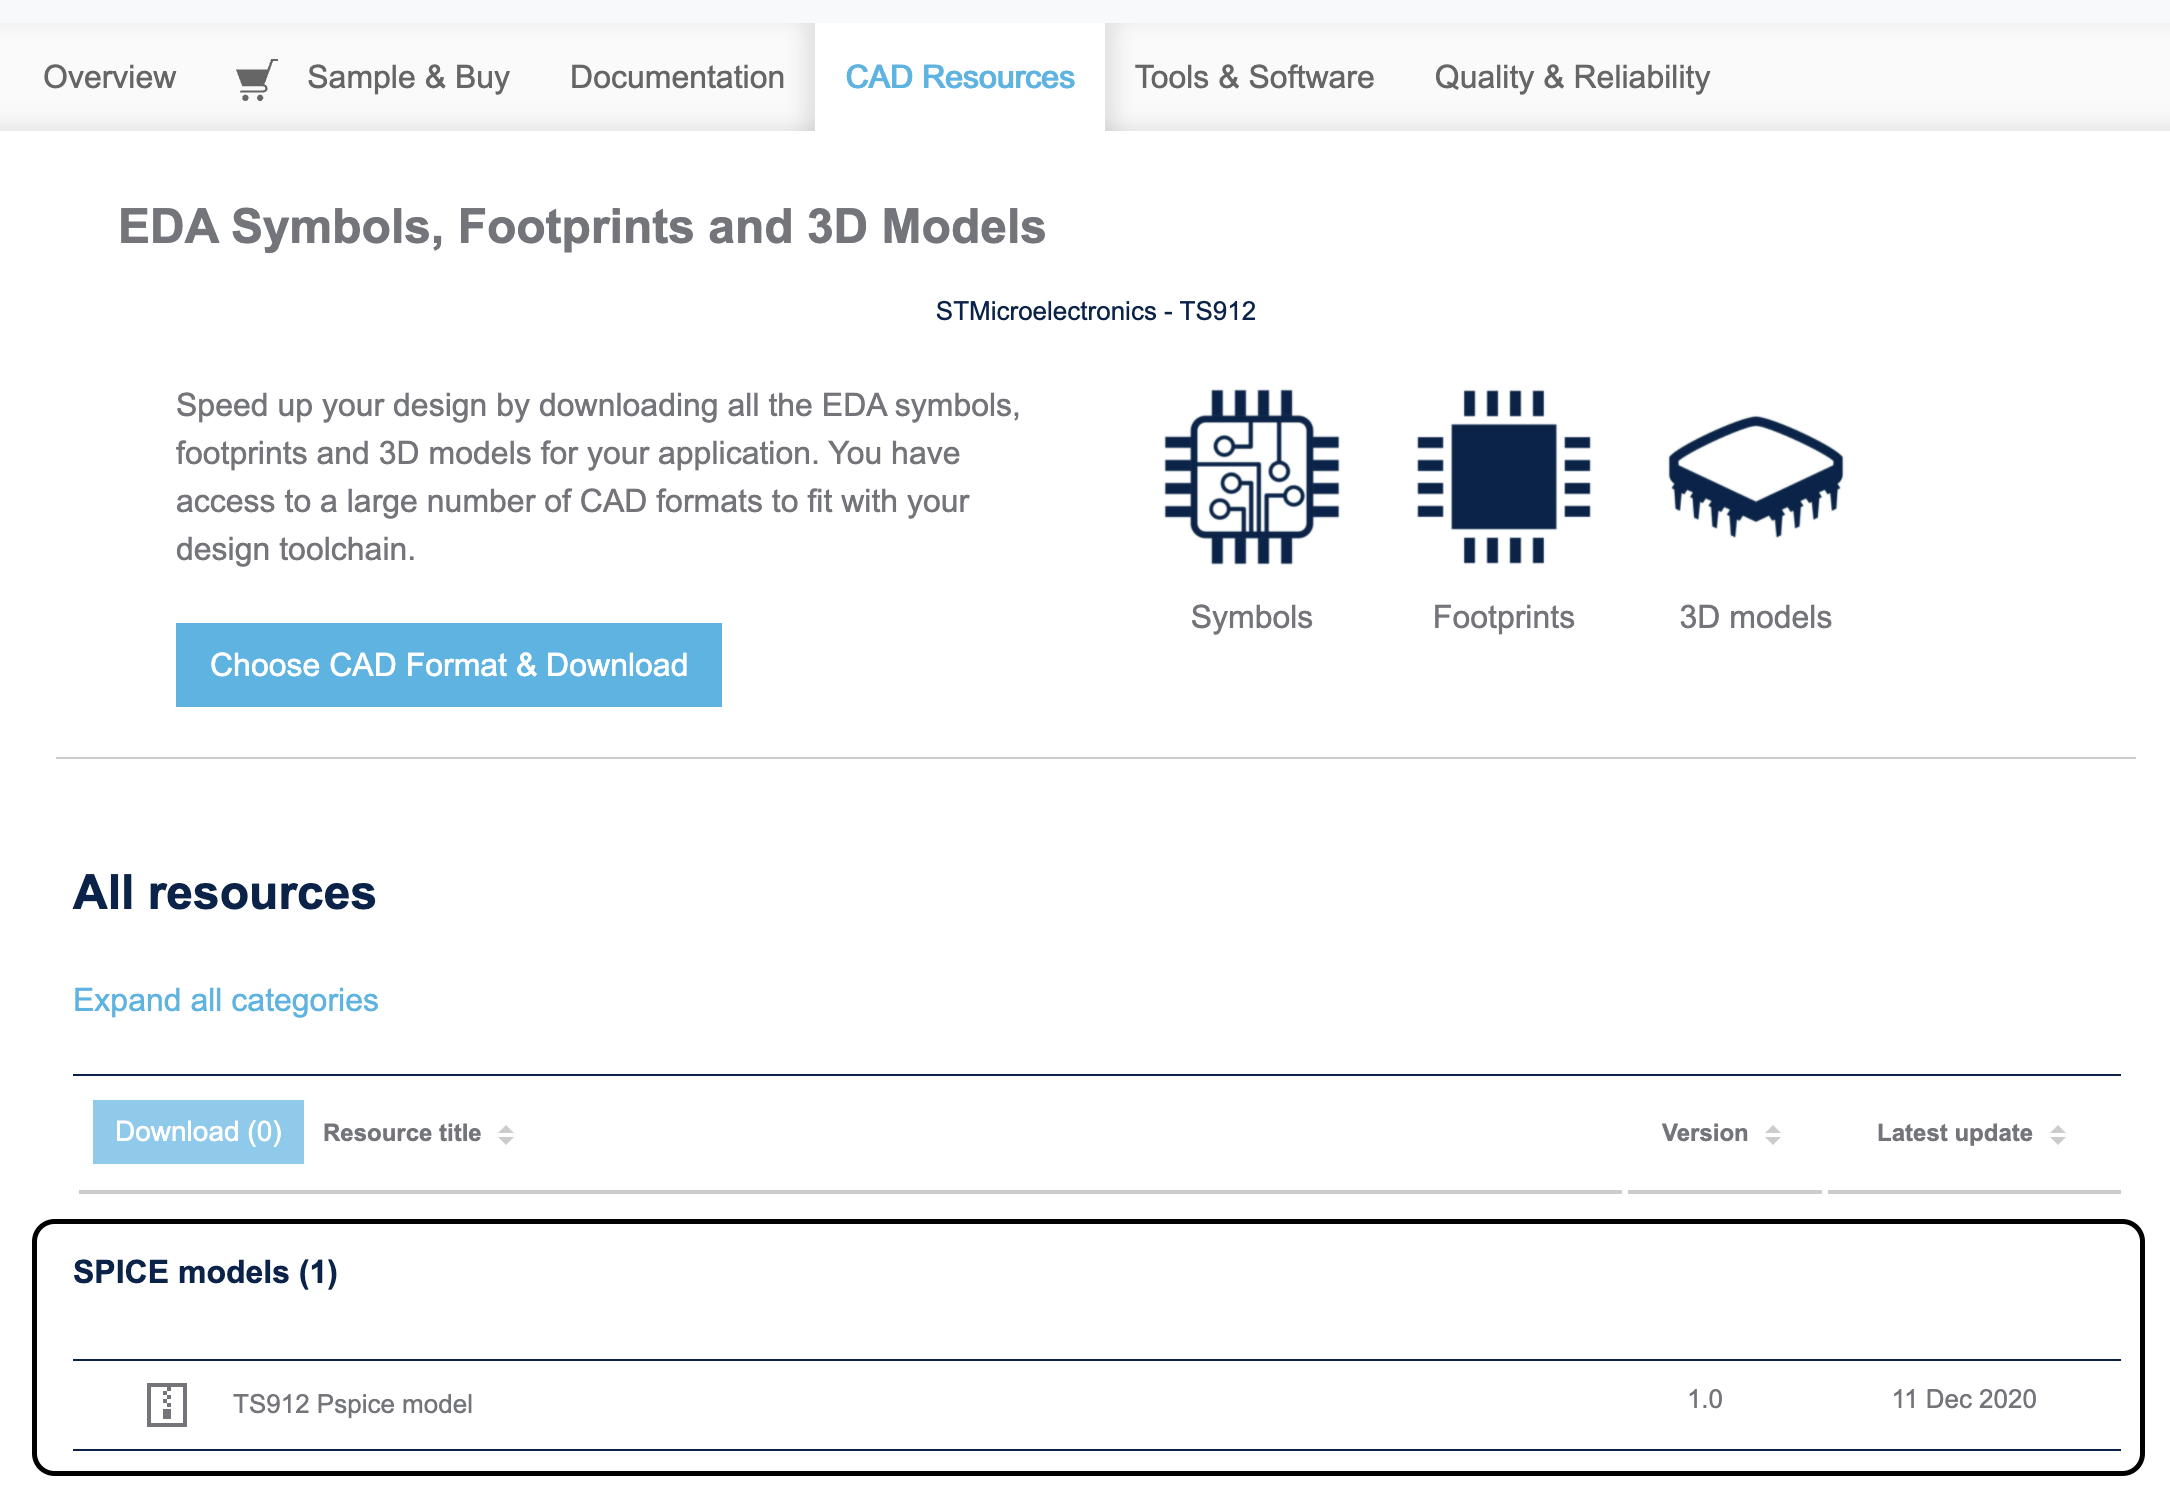
\includegraphics[width=\linewidth]{pictures/spice_model_search2.png}
              \end{minipage} 
        \end{tabular}
      \end{table}
      \end{tiny} \end{spacing}

\end{frame}

\begin{frame}[t]{Subscircuit erstellen} 

    Ein spice Model ist eine einfache Text-Datei, die einfach in LTSpice eingebunden werden kann.
    Kopiert den \textbf{subcircuit} dazu in eine Text-Datei mit der Endung .sub \textbf{TS912.sub} und speichert diese im Ordner:

    \begin{scriptsize}
        \begin{enumerate}
            \item Windows \textbf{C:/Users/"USER"/Documents/LTspiceXVII/lib/sub}
            \item MacOS \textbf{/Users/"user"/Library/ApplicationSupport/LTspice/lib/sub}.
        \end{enumerate}
    \end{scriptsize}

    \begin{spacing}{0.9} \begin{tiny}
        \begin{minipage}{\textwidth}
          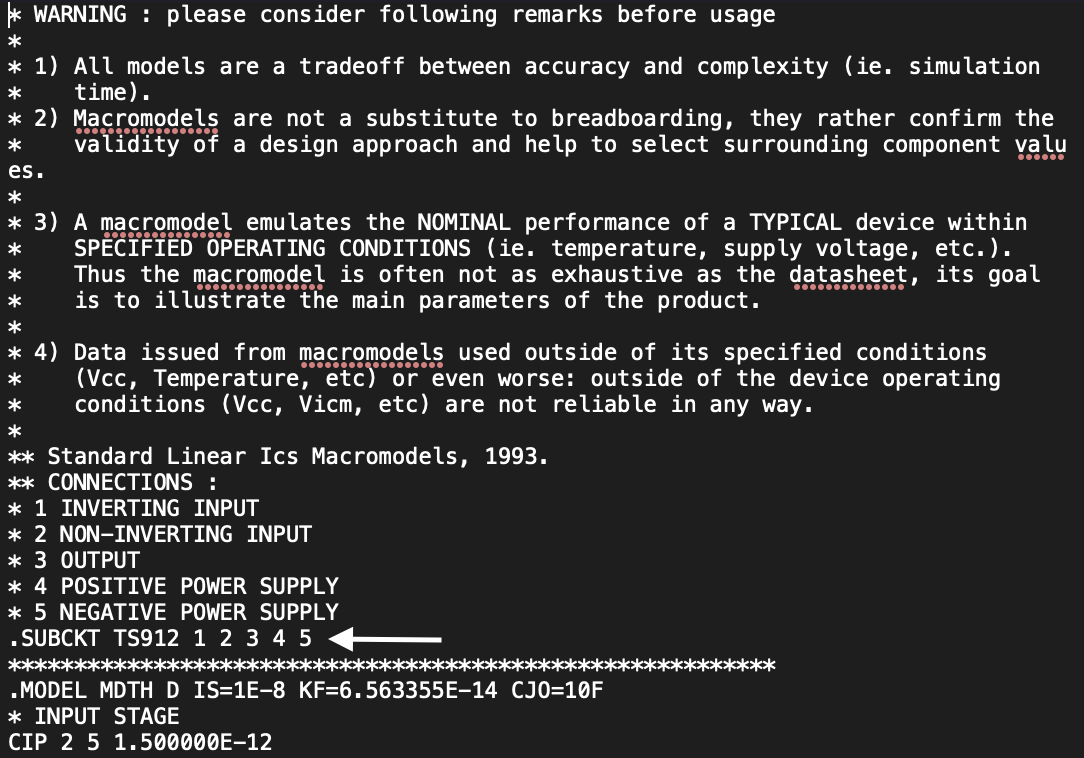
\includegraphics[width=0.5\linewidth]{pictures/spice_model.png}
        \end{minipage}
    \end{tiny} \end{spacing}
\end{frame}

\begin{frame}[t]{LTSpice Symbol erstellen} 

    \begin{enumerate}
        \item Öffnet LTspice und öffnet das soeben erstellte File. 
        \item Mac: More Choices -\> Open Other Type of File
        \item Windows: Drag and Drop der Datei in LTspice
        \item Jetzt markiert ihr die Zeile mit dem \textbf{.subckt} klickt ihr mit der rechten Maustaste
        \item Klickt nun auf "Create Symbol"
    \end{enumerate}


    \begin{spacing}{0.9} \begin{tiny}
        \begin{minipage}{\textwidth}
          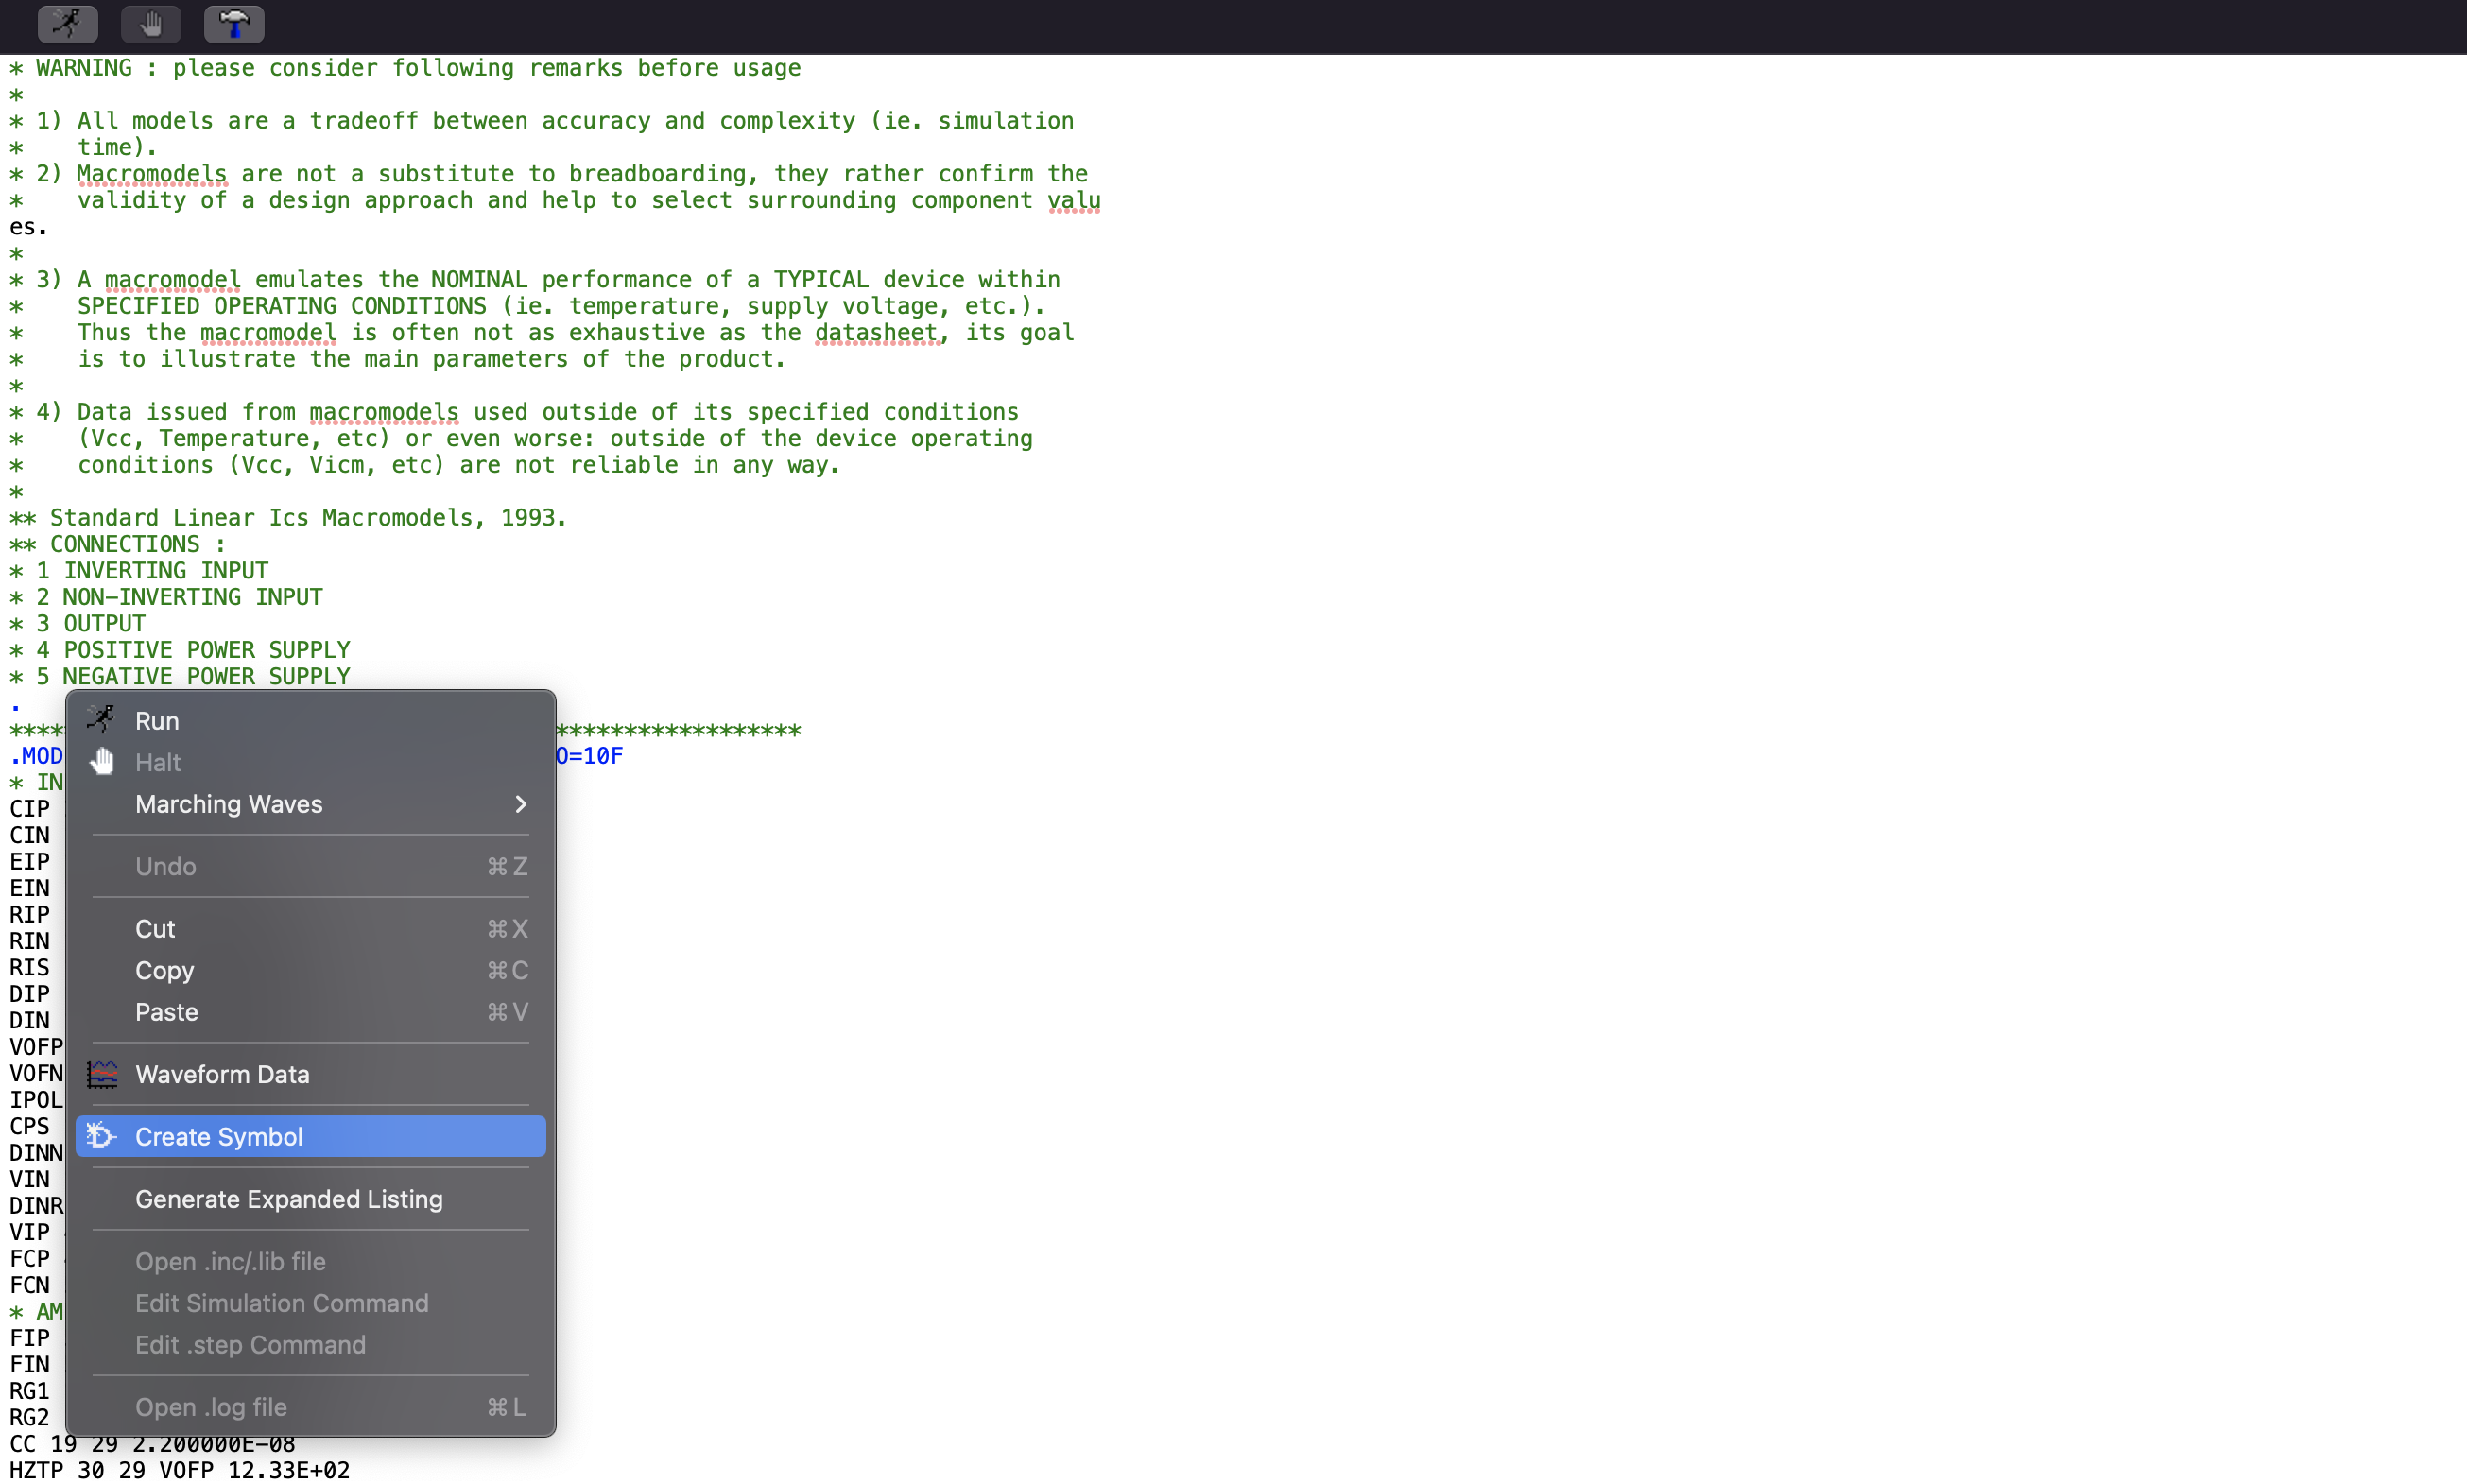
\includegraphics[width=0.6\linewidth]{pictures/ModelCreation.png}
        \end{minipage}
    \end{tiny} \end{spacing}

\end{frame}


\begin{frame}[t]{LTSpice Symbol modellieren 1} 

    Nun könnt ihr hier über das Zeichentool kreativ werden.
    Wichtig ist, dass ihr die Symbol Attribute korrekt einstellt. Ihr kommt in
    die Attribut Dialog über (Edit -\> Attributes) .Die Pin Nummerierung muss 
    mit der im subcircuit übereinstimmen, klickt mit der rechten Maustate auf einen Pin.
    Die Benamung der Pins könnt ihr natürlich auch ändern.

    \begin{spacing}{0.9} \begin{tiny}
        \begin{minipage}{\textwidth}
          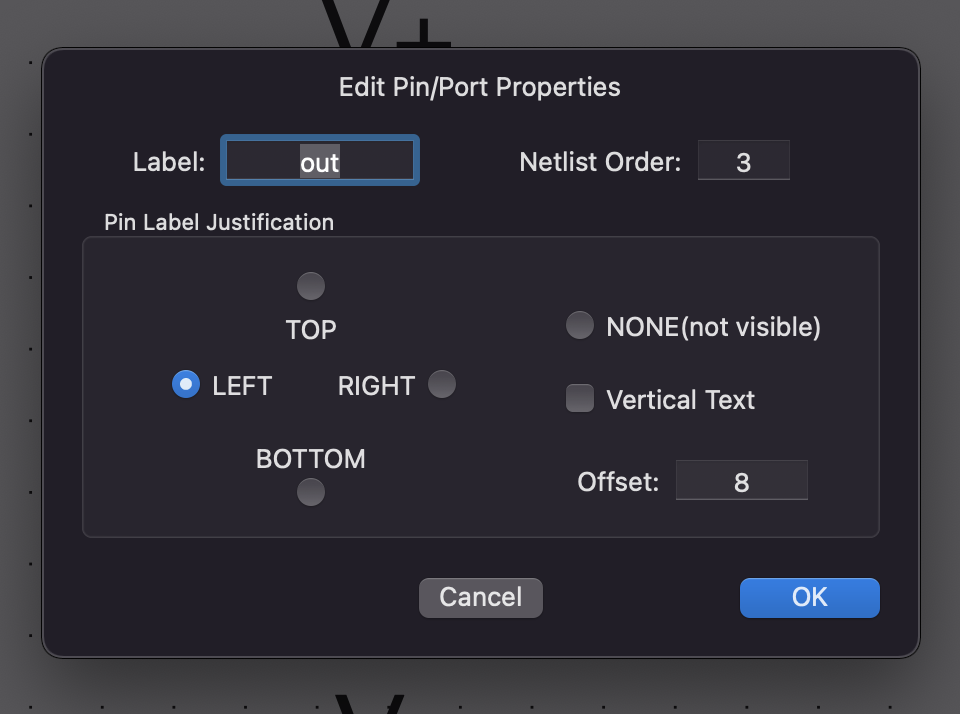
\includegraphics[width=0.6\linewidth]{pictures/pinNummerierung.png}
        \end{minipage}
    \end{tiny} \end{spacing}

\end{frame}


\begin{frame}[t]{LTSpice Symbol modellieren 2}

    Zudem müssen wir in LTspice den Bezug zum subcircuit definieren. Dazu stellt ihr sicher, dass die
    Variable ModelFile auf unser zuvor gespeichertes File zeigt. (TS912.sub)

    \begin{spacing}{0.9} \begin{tiny}
        \begin{minipage}{\textwidth}
          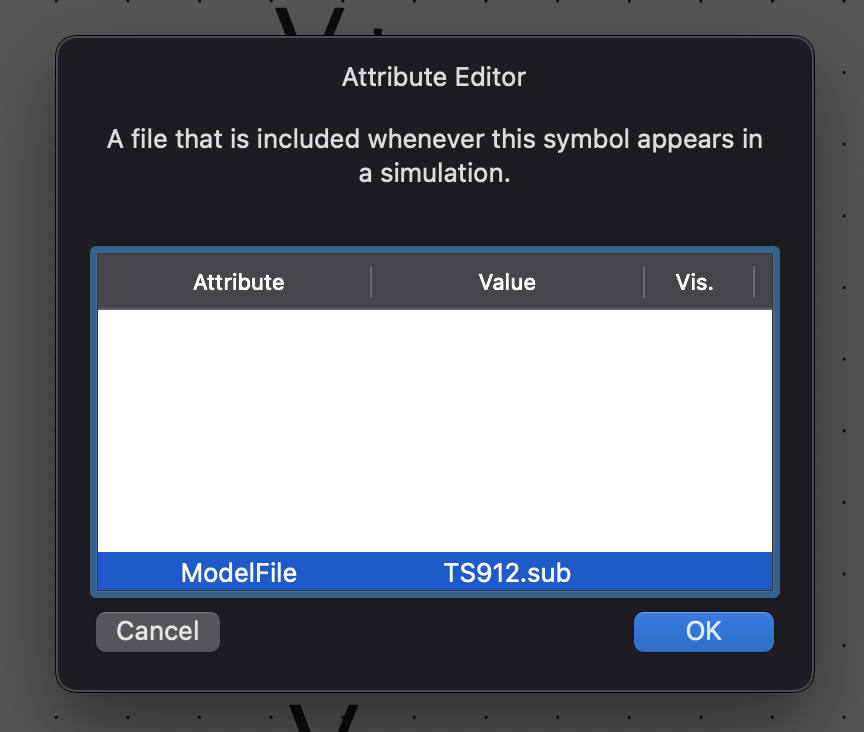
\includegraphics[width=0.6\linewidth]{pictures/spiceModel.png}
        \end{minipage}
    \end{tiny} \end{spacing}

\end{frame}

\begin{frame}[t]{Bauteil verwenden}

    Wir haben nun:

    \begin{enumerate}
        \item Einen subcircuit heruntergeladen
        \item Ihn unter dem Namen TS912.sub im \textbf{sub} Ordner von LTspice gespeichert
        \item Aus dem subscircuit ein Symbol erstellt
        \item Dieses Symbol angepasst und zum subcircuit verlinkt
    \end{enumerate}

    Jetzt können wir über den Bauteileditor (F2) im Menü \textbf{AutoGenerated}, unseren
    TS912 laden und in LTspice verwenden.

    \textbf{Hint: Bei einem Mac müsst ihr nach dem Erstellen einmal neu starten.}

\end{frame}